\label{Chapter3}

\chapter{A tool for Ethereum analytics}
In this chapter we describe in details how our created tool works. First of all, we describe its architecture in details, highlighting every separated part, in particular we talk about \textit{Parity}, \textit{Web3J} and \textit{JSON-RPC}. Further, we discuss some case studies using our tool, retrieving data from Ethereum blockchain, and then combining it with external data. Furthermore, we discuss about tool implementation, and how it works internally.
\section{Tool architecture}
In this section we will describe how this tool works. This tool is build for create a custom view of either the Ethereum blockchain or the Bitcoin blockchain.
\newline 
Since we do not use Bitcoin blockchain, we will describe only how the Ethereum part works. We said the the view is \textit{custom} because this tool allows the user to extract whatever he needs from the blockchain, such as:
\begin{itemize}
    \item Blocks information, e.g. block number, block hash;
    \item Transactions information, e.g. transaction hash, sender, receiver, created contract (if exists);
    \item Contract internal transactions information, e.g. transaction hash, sender, receiver, father transaction hash (the transaction that calls the defined contract)
\end{itemize}

Furthermore, the view \textit{customization} is possible because our tool is able to retrieve \textbf{external data} (for external we mean data not stored directly inside blockchain) and combine it with blockchain's internal data. This external data could be of any nature, e.g. exchange rates, ICOs data, \textit{etc...}.

The image in the next page shows how out tool works. %Cambiare immagine, aggiungere anche i dati esterni
\begin{center}
    \[
        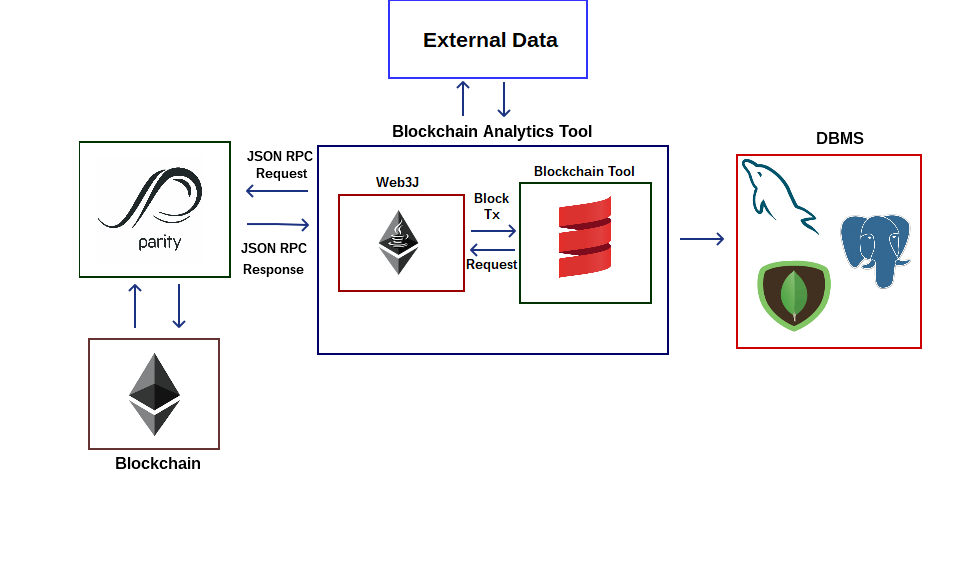
\includegraphics[
            trim=1cm 3cm 1cm 1cm,
            width=0.85\columnwidth,]{architecture_total.png}
    \]
\end{center}
As you can see, in order to retrieve blockchain data, our tool makes a request through Web3J (described in \ref{web3j}), which in turn makes a request directly to the Ethereum client, in our case Parity (described in \ref{parity}). This requests are made using the JSON-RPC protocol (described in \ref{jsonrpc}). 

When Parity returns the wanted result, Web3J serialize it into a collection of objects, then returns them to our tool. Since these classes do not contains all information, we decided to wrap them in another classes, retrieving all missing information, i.e. contract internal trasactions.

In the next subsections, we briefly describe how Parity, Web3J and JSON RPC work. Then, in the next sections, we show some view examples, using \textit{MongoDB} as DBMS.

\subsection{Parity}
\label{parity}
\href{https://www.parity.io/}{Parity} \cite{authors2017ethereum} is an Ethereum client, written from the ground-up for correctness-verifiability, modularisation, low-footprint and high-performance. \newline
To this end it utilises the Rust language, a hybrid imperative/OO/functional language with an emphasis on efficiency. 
\newline
Parity comes with an extensive, in-built Ethereum Wallet and DApp environment. It includes:
\begin{itemize}
    \item Account, address-book and multi-sig management.
    \item Key creation, importing and exporting.
    \item Web3 Ðapp browser.
    \item Hardware and electronic cold-wallet support.
    \item Name registry support.
    \item Contract development, deployment and interaction environment.
\end{itemize}

\subsection{Web3J}
\label{web3j}
\href{https://web3j.io/}{Web3J} is a highly modular, reactive, type safe Java and Android library for working with Smart Contracts and integrating with clients (nodes) on the Ethereum network. This allows to work with the Ethereum blockchain, without the additional overhead of having to write an integration code for the platform.

Web3J is capable to connect to a local blockchain, downloaded using Parity, \href{https://github.com/ethereum/go-ethereum/wiki/geth}{Geth} or another Ethereum client, or a remote one, like \href{https://infura.io}{Infura}.
In order to retrieve blockchain data, Web3J uses a protocol called JSON-RPC, which will be described in section \ref{jsonrpc}. 

\subsection{JSON-RPC}
\label{jsonrpc}
JSON-RPC \cite{json2012json} is a remote procedure call protocol encoded in JSON. It is a very simple protocol (and very similar to XML-RPC), defining only a few data types and commands. JSON-RPC allows for notifications (data sent to the server that does not require a response) and for multiple calls to be sent to the server which may be answered out of order.

JSON-RPC works by sending a request to a server implementing this protocol. The client in that case is typically software intending to call a single method of a remote system. Multiple input parameters can be passed to the remote method as an array or object, whereas the method itself can return multiple output data as well. (This depends on the implemented version).

All transfer types are single objects, serialized using JSON. A request is a call to a specific method provided by a remote system. It must contain three certain properties:
\begin{itemize}
    \item \textit{Method}: A String with the name of the method to be invoked;
    \item \textit{Params}: An Object or Array of values to be passed as parameters to the defined method;
    \item \textit{Id}: A value of any type used to match the response with the request that it is replying to.
\end{itemize}

The receiver of the request must reply with a valid response to all received requests. A response must contain the following properties:
\begin{itemize}
    \item \textit{Result}: The data returned by the invoked method. If an error occurred while invoking the method, this value must be null;
    \item \textit{Error}: A specified error code if there was an error invoking the method, otherwise null;
    \item \textit{Id}: The id of the request it is responding to.
\end{itemize}
Since there are situations where no response is needed or even desired, notifications were introduced. A notification is similar to a request except for the id, which is not needed because no response will be returned. In this case the id property should be omitted (Version 2.0) or be null (Version 1.0).
\subsubsection{Examples}
In this subsection, we will show one example of \textit{Request and Response} and one of \textit{Notification} using JSON-RPC version 2.0.
\newline
Request and response:
\begin{lstlisting}[language=json]
Request
{
    "jsonrpc": "2.0", 
    "method": "subtract", 
    "params": {
                "minuend": 42, 
                "subtrahend": 23
              },
    "id": 3
}
Response 
{
    "jsonrpc": "2.0", 
    "result": 19, 
    "id": 3
}
\end{lstlisting}
Notification, with no response
\begin{lstlisting}[language=json]
{
    "jsonrpc": "2.0",
    "method": "update",
    "params": [1,2,3,4,5]
}
\end{lstlisting}

\section{External Information Sources}
\label{informationsources}
\subsection{ICO-Rating}
\label{icoRating}
\subsubsection{Available Data}
\label{icoRatingAvailableData}
\href{https://icorating.com/}{ICO-Rating} contains a list of active ICOs. It rates them relying on they stability and risk on investment. ICORating rates an ICO using three scores:
\begin{itemize}
    \item \textit{\textbf{HypeScore}}: Hype-score shows investor level of interest in the project. The higher the score, the more people may consider the project for future investments. That is a numeric score between 0 and 5;
    \item \textit{\textbf{RiskScore}}: Risk score is aimed at assessing the risk of potentially fraudulent activities. The higher the risk score, the less information there is on the details of the ICO campaign, product development, the team and the documentation, which calls into question the possibility for success of the start-up and the ICO/Token sale. That is a numeric score between 0 and 5;
    \item \textit{\textbf{Investment Rating}}: The metrics of this parameter is divided into 10 levels: \textit{Positive+, Positive, Stable+, Stable, Risky+, Risky, Risky-, Negative, Negative-, Default}. The higher the rate assigned to the project, the better the overall quality of the project’s documentation, and the lower the number of risks for future investors.
\end{itemize}
\subsubsection{Extracted API Methods}
In this subsection we describe the API internal methods that retrieve data listed in \ref{icoRatingAvailableData}. \newline 
In the following table is written that the methods used to retrieve all the data described above take only the token name as input. \newline
This is because ICORating does not have a REST API, or any other API to call, but we had to do a scraping on the HTML page at the address \texttt{icorating.com/ico/<token-name>/}. \newline

In order to retrieve all this data, we created a class called \textbf{ICORatingAPI}, following are the methods in this class.
\begin{center}
\begin{tabular}{| C{2.5cm} | C{4cm} | C{5.5cm} |} \hline
    \textit{Field Name} & \textit{Description} & \textit{Method Signature}\\ \hline 
    \textbf{Hype Score} & ICORating's hype score for the given ICO & \texttt{getHypeScore(icoName)}\\ \hline 
    \textbf{Risk Score} & ICORating's risk score for the given ICO & \texttt{ getRiskScore(icoName)}\\ \hline 
    \textbf{Investment Rating} & ICORating's investment rating for the given ICO & \texttt{getInvestmentRating(icoName)}\\ \hline 
\end{tabular}
\end{center}

\subsection{ICOBench}
\label{icoBench}
\subsubsection{Available Data}
\href{https://icobench.com/}{ICOBench} is a free ICO rating platform and a blockchain community supported by a wide range of experts that provides analytical, legal, and technical insights to the investors.
ICOBench also gives a rating for each Token. Rating is given in combination of:
\begin{itemize}
    \item Their assessment algorithm that uses more than 20 different criteria on which each ICO can earn more than 30 points and
    \item The rating the independent experts give to the ICO following our rating methodology suggestions.
\end{itemize} 

The rating is a float value beetween 0 and 5.0 and is splitted in four subratings, which are combined (with a simple arithmetic average) to retrieve the general ICO rating:
\begin{itemize}
    \item ICO Profile
    \item Team
    \item Vision
    \item Product
\end{itemize}
ICOBench gives an useful \href{https://icobench.com/developers}{REST API} to retrieve all data they have about 1787 ICO from 164 different countries. \newline
Like ICORating in \ref{icoRating}, in order to retrieve all needed data with rest APIs, we have to use  either the token name or the token symbol. We have to do this because ICOBench does not store (or does not make available) the contract address, which we believe is more unambiguous then token name. \newline
In the next subsection we will talk about all the data that we extracted using this API.
\subsubsection{Extracted API Methods}

In order to extract useful data using this API, we have created a specific class, called \textbf{ICOBenchAPI}, following are the methods in this class.
\begin{center}
\begin{tabular}{| C{2cm} | C{4cm} | C{7cm} |} \hline
    \textit{Field Name} & \textit{Description} & \textit{Method Signature}\\ \hline 
    \textbf{ICO Symbol} & ICO's symbol & \texttt{getSymbol(icoName)}\\ \hline 
    \textbf{Exchange Details} & Details about the Exchanges that trade this token & \texttt{getExchanges(icoName/icoSymbol)}\\ \hline 
    \textbf{Market Cap} & Actual Market Capitalization of the given ICO &
    \texttt{getMarketCap(icoName/icoSymbol)}\\ \hline
    \textbf{General Rating} & ICOBench's general rating for the given Token &
    \texttt{getGeneralRating(icoName/icoSymbol)
    }\\ \hline
    \textbf{Profile Rating} & ICOBench's profile rating for the given Token &
    \texttt{getProfileRating(icoName/icoSymbol)}\\ \hline 
    \textbf{Team Rating} & ICOBench's team rating for the given Token &
    \texttt{getTeamRating(icoName/icoSymbol)}\\ \hline 
    \textbf{Vision Rating} & ICOBench's vision rating for the given Token ICO &
    \texttt{getVisionRating(icoName/icoSymbol)}\\ \hline 
    \textbf{Product Rating} & ICOBench's product rating for the given Token &
    \texttt{getProductRating(icoName/icoSymbol)}\\ \hline
\end{tabular}
\end{center}

\subsection{TokenWhoIs}
\subsubsection{Available Data}
\href{https://tokenwhois.com/}{TokenWhoIs} is a website that contains a wide list of ICOs, and for eeach of them, it contains information like Market Capitalization, used blockchain, unit price in various currencies. \newline
Like ICOBench in \ref{icoBench} in order to retrieve all needed data with rest APIs, we have to use  either the token name or the token symbol. 
\subsubsection{Extracted API Methods}
In order to extract useful data using this API, we have created a specific class, called \textbf{TokenWhoIsAPI}, following are the methods in this class.
\begin{center}
\begin{tabular}{| C{2cm} | C{4cm} | C{7cm} |} \hline
    \textit{Field Name} & \textit{Description} & \textit{Method Signature}\\ \hline 
    \textbf{Used Blockchain} & Blockchain used by the given token & \texttt{getUsedBlockchain(icoName)}\\ \hline 
    \textbf{Market Cap} & Actual Market Capitalization of the given ICO &
    \texttt{getMarketCap(icoName)}\\ \hline
    \textbf{Token Unit Price (USD)} & Token current unit price (USD) &
    \texttt{getUSDUnitPrice(icoName)
    }\\ \hline
    \textbf{Token Unit Price (ETH)} & Token current unit price (ETH) &
    \texttt{getETHUnitPrice(icoName, icoSymbol)}\\ \hline 
    \textbf{Token Unit Price (BTC)} & Token current unit price (BTC) &
    \texttt{getBTCUnitPrice(icoName)}\\ \hline 
    \textbf{Exchange Names} & Name of Exchanges that trade this token ICO &
    \texttt{getExchangeNames(icoName)}\\ \hline 
    \textbf{Token Supply (USD)} & Token total supply in USD &
    \texttt{getUSDSupply(icoName,icoSymbol)}\\ \hline
\end{tabular}
\end{center}

\subsection{CoinMarketCap}
\href{https://coinmarketcap.com/}{CoinMarketCap} is a website that provides market data about cryptocurrencies and ICO tokens. It provides data like actual and historical market capitalization and actual and historical cryptocurrency unit price in various currencies.
\subsubsection{Available Data}
CoinMarketCap provides an useful REST API, which prvides the following data for each cryptocurrency:
\begin{itemize}
    \item \textit{Name}: Token Name;
    \item \textit{Symbol}: token Symbol;
    \item \textit{Price USD}: Current currency unit price in USD;
    \item \textit{Price BTC}: Current currency unit price in BTC;
    \item \textit{24h volume USD}: Volume of currency transferred in the last 24 hours, in USD;
    \item \textit{Market Cap USD}: Coin Market Capitalization in USD;
    \item \textit{Available Supply}: Coin available supply. 'Available' means 'available to buy';
    \item \textit{Total Supply}: Coin total supply;
    \item \textit{Percent Change 1h}: Change of coin price in the last hour;
    \item \textit{Percent Change 24h}: Change of coin price in the 24 hours;
    \item \textit{percent Change 7d}: Change of coin price in the seven days;
    \item \textit{Last Updated}: Last time these information were updated.
\end{itemize}
\subsubsection{Extracted API Methods}
In order to extract useful data using this API, we have created a specific class, called \textbf{CoinMarketCapAPI}, following are the methods in this class.
\begin{center}
\begin{tabular}{| C{2cm} | C{4cm} | C{7cm} |} \hline
    \textit{Field Name} & \textit{Description} & \textit{Method Signature}\\ \hline 
    \textbf{Market Cap} & Actual Market Capitalization of the given token &
    \texttt{getTokenMarketCap(icoName, icoSymbol)}\\ \hline
    \textbf{Token Unit Price (USD)} & Token current unit price (USD) &
    \texttt{getTokenUSDPrice(icoName, icoSymbol)}\\ \hline
    \textbf{Token Unit Price (BTC)} & Token current unit price (BTC) &
    \texttt{getTokenBTCPrice(icoName, icoSymbol)}\\ \hline 
    \textbf{Exchange Names} & Name of Exchanges that trade this token ICO &
    \texttt{getExchangeNames(icoName)}\\ \hline 
    \textbf{Token Supply (USD)} & Token total supply in USD &
    \texttt{getUSDSupply(icoName,icoSymbol)}\\ \hline
\end{tabular}
\end{center}

\subsection{EtherScan}
\label{etherscan}
\subsubsection{Available Data}
\href{https://etherscan.io/}{EtherScan} is a Block Explorer and Analytics Platform for Ethereum.
It provides a view of all blockchain containing:
\begin{itemize}
    \item Block information such as block number, hash, miner;
    \item Accounts information;
    \item Transaction information such as hash, receiver, sender, amount;
    \item Internal Transaction information such as hash, receiver, sender, amount, father transaction's hash;
    \item Tokens information such as token name, symbol, owners;
\end{itemize}
Etherscan also provides an useful REST API to retrieve all data they have. In the next section we'll describe all data extracted from Etherscan
\subsubsection{Extracted API Methods}
In order to extract useful data using this API, we have created a specific class, called \textbf{EtherScanAPI}, following are the methods in this class.
\begin{center}
\begin{tabular}{| C{2cm} | C{4cm} | C{7cm} |} \hline
    \textit{Field Name} & \textit{Description} & \textit{Method Signature}\\ \hline 
    \textbf{Token total Supply } & Token total supply &
    \texttt{getTotalSupplyByAddress(icoAddress)}\\ \hline
    \textbf{Token balance by adderess} & Given an account address, it returns its token balance &
    \texttt{getTokenAccountBalance(icoAddress, accountAddress)}\\ \hline
\end{tabular}
\end{center}

\subsection{Ethplorer}
\subsubsection{Available Data}
\href{https://ethplorer.io/}{Ethplorer} is a token blobkchain explorer. For each token, it provides information such as:
\begin{itemize}
    \item Basic token information (Name, Symbol, Price, Total Supply);
    \item Basic token contract information (Address, creator's address, balance (ETH), number of transactions);
    \item Token Operations details inside a time interval (Transaction hash, sender, receiver, amount of token transferred);
\end{itemize}
\subsubsection{Extracted API Methods}
In order to extract useful data using this API, we have created a specific class, called \textbf{EthplorerAPI}, following are the methods in this class.
\begin{center}
\begin{tabular}{| C{2cm} | C{4cm} | C{7cm} |} \hline
    \textit{Field Name} & \textit{Description} & \textit{Method Signature}\\ \hline
    \textbf{ICO Name} & ICO's name & \texttt{getTokenName(contractAddress)}\\ \hline 
    \textbf{ICO Symbol} & ICO's Symbol & \texttt{getTokenSymbol(contractAddress)}\\ \hline 
    \textbf{Token Price} & Token current price (USD) & \texttt{getTokenPrice(contractAddress)}\\ \hline
\end{tabular}
\end{center}

\section{Implementation}
In this section we will explain in details the implementation of the tool, built to retrieve blockchain data and other external data and combine them.

This tool is written in Scala Programming Language and built with Scala Build Tool (SBT). Scala has been chosen because, since it's compiled in bytecode that runs on Java Virtual Machine (JVM), it can be combined with Java external libraries without any problem. \newline
Thanks to this property, it was possible to use Web3J (explained in \ref{web3j}) library to retrieve blockchain data. It is a Java and Android library for working with Smart Contracts and integrating with clients (nodes) on the Ethereum network.

The core class, used to access both \textit{Ethereum} and \textit{Bitcoin} blockchain is \texttt{BlockchainLib}. It has two methods:
\begin{itemize}
    \item \texttt{getBitcoinBlockchain(settings: BitcoinSettings)}
    \item \texttt{getEthereumBlockchain(url: String)}
\end{itemize}
Since for this thesis we used only \texttt{getEthereumBlockchain}, we will describe only this class. 
\newline
The \texttt{getEthereumBlockchain} method takes one parameter that is the url where the blockchain is stored.
For example, if you are using Parity locally, the url should be like \texttt{http://localhost:8545}, since the \texttt{8545} port is the default port where Parity listens to JSON-RPC requests.

This method returns an istance of \texttt{EthereumBlockchain} which extends a \texttt{Traversable}, so it can be looped with a simple \texttt{foreach}, setting first the following parameters:
\begin{itemize}
    \item \textit{startBlock}: the block from which to start. It is modifiable with the \texttt{setStart} method. If not setted, the default is 0;
    \item \textit{endBlock}: the block from which to end. It is modifiable with the \texttt{setEnd} method. If not setted, the default is the last block;
    \item \textit{step}: the interval between each block visited. It is modifiable with the \texttt{setStep} method. If not setted, the default is 1.
\end{itemize}

This \texttt{foreach} loops over all requested block. Each block is an instance of the \texttt{EthereumBlock} class. An \texttt{EthereumBlock} object is retrieved from an \texttt{EthBlock.Block} object of the \textit{Web3J} library, retrieved calling the \texttt{Web3J.getBlockByNumber} method. This \textit{Web3J}'s method does internally a JSON-RPC request to the \textit{getBlockByNumber} method, directly to Parity, at the previously defined url.
\newline
The difference between the \texttt{EthereumBlock} object and the \texttt{EthBlock.Block} object is that the first one contains also the internal transactions information, not normally returned using an implemented method in \textit{Web3J}. \newline
In order to retrieve all information about Contract Internal Transaction, we have to do anther JSON-RPC request calling the \textit{trace\_block} method. This request allows to see all the transactions and internal transactions contained in this block. From this request, we extract only the internal transactions, filtering the normal transactions, already known.
\newline
Each \texttt{EthereumBlock} object contains the following information:
\begin{itemize}
    \item \textit{number}: block number inside blockchain;
    \item \textit{hash}: block hash;
    \item \textit{parentHash}: hash of the parent block;
    \item \textit{miner}: address of the account that mined this block;
    \item \textit{size}: size of block in bytes;
    \item \textit{timeStamp}: the unix timestamp for when the block was collated;
    \item \textit{transactions}: Array of transaction objects (this data structure will be described below);
    \item \textit{internalTransactions}: Array of contract transaction objects (this data structure will be described blow).
\end{itemize}

The \textit{transaction} field is a List of \texttt{EthereumTransaction} objects. These objects are created using a factory method that takes as input a object of \texttt{EthBlock.TransactionObject} \textit{Web3J} class. 
\newline
Each \texttt{EthereumTransaction} object contains the following information:
\begin{itemize}
    \item \textit{hash}: transaction hash;
    \item \textit{blockHash}: hash of the block that contains this transaction;
    \item \textit{transactionIndex}: index of the transaction inside its block;
    \item \textit{from}: transaction sender;
    \item \textit{to}: transaction receiver;
    \item \textit{value}: value transferred in this transaction in Wei;
    \item \textit{gasPrice}: gas price provided by the sender in Wei;
    \item \textit{gas}: gas provided by the sender;
    \item \textit{input}: the data send along with the transaction;
    \item \textit{creates}: creates contract hash. This field is not null if and only if this transaction creates a contract, which address is displayed here;
\end{itemize}
The \textit{internalTransactions} field is a List of \texttt{EthereumInternalTransaction} objects. These objects are created unmarshalling the result of the  \textit{trace\_block} JSON-RPC request. \newline
Each \texttt{EthereumInternalTransaction} object contains the following information:
\begin{itemize}
    \item \textit{parentTxHash}: hash of the parent transaction;
    \item \textit{txType}: transaction type (create, suicide, call);
    \item \textit{from}: transaction sender;
    \item \textit{to}: transaction receiver;
    \item \textit{value}: value transferred in this transaction in Wei.
\end{itemize}

These classes envelop all the Ethereum Blockchain's useful data. In order to retrieve external data (e.g. ICO data), we have to create one new class inside the \texttt{custom} package.
\newline
Let's consider the section \ref{exchangerates} as an example. In order to retrieve the exchange rate information, we created a new class called \texttt{custom.PriceHistorical} with one method, called \texttt{getPrice} which takes one argument as input that is the date timestamp, and returns the ETH/USD exchange rate in that timestamp.

When all the data is prepared to be gathered, you must choose what kind of database you will use. This tool supports both SQL (MySQL, PostgreSQL) and NoSQL (MongoDB) databases.
If you want to use a \textbf{SQL} database, you have to use our \texttt{db} package, designed to be used in these cases. More precisely, you have to instantiate an object of the \texttt{Table} class, that is a table in the SQL database. 
\newline
Here's an exhaustive example:
\begin{lstlisting}[language=Scala]
    import tcs.db.sql.Table
    import tcs.db.{DatabaseSettings, PostgreSQL}
    val blockTable = new Table(
      sql"""
          SQL COMMAND TO CREATE TABLE
         """,
      sql"""
           SQL COMMAND TO INSERT ELEMENT IN TABLE
         """,
      new DatabaseSettings(dbName, PostgreSQL)
    )
\end{lstlisting}
If you want to use a \textbf{NoSQL} database, you have to use our \texttt{mongo} and \texttt{db} packages, designed to be used in these cases. More precisely, you have to instantiate an object of the \texttt{Collection} class, then call this \texttt{append} method to add elements inside the collection. 
\newline
Here's an example:
\begin{lstlisting}[language=Scala]
    import mongo.Collection
    import db.{DatabaseSettings, MongoDB}
    val collection = new Collection(
        "collectionName", 
        new DatabaseSettings("dbName", MongoDB)
    )
    //Data Gathering
    collection.append(gatheredData)
\end{lstlisting}

\section{Case study: a basic view of the blockchain}
This view contains data about all transactions (and, contract internal transactions) that has been done inside Ethereum blockchain. The fields in this view are the following:
\begin{itemize}
    \item \textit{\textbf{txHash}}: transaction hash;
    \item \textit{\textbf{blockHeight}}: block number of the block that contains this transaction;
    \item \textit{\textbf{txIndex}}: transaction progressive number inside its block;
    \item \textit{\textbf{date}}: the date when block is mined;
    \item \textit{\textbf{from}}: transaction sender (the address of who is transferring money or creating a contract);
    \item \textit{\textbf{to}}: transaction receiver (the address of who is receiving money, this field is empty if this transaction creates a contract);
    \item \textit{\textbf{value}}: how much (in ETH) is transferred;
    \item \textit{\textbf{creates}}: the address of the newly created contract (empty if this transaction does not create a contract);
    \item \textit{\textbf{internalTransactions}}: contains all the internal transactions generated by this transaction, it's a list of objects containing the following fields:
        \subitem \textit{\textbf{parentTxHash}}: hash of the father transaction (the transaction that generates this one);
        \subitem \textit{\textbf{txType}}: internal transaction type (call, suicide, create);
        \subitem \textit{\textbf{from}}: internal transaction sender;
        \subitem \textit{\textbf{to}}: internal transaction receiver;
        \subitem \textit{\textbf{value}}: how much (in ETH) in transferred.
\end{itemize}
Here's the code snippet used to create this view:
\begin{lstlisting}[language=Scala]
    val blockchain = BlockchainLib.getEthereumBlockchain("http://localhost:8545")
      val mongo = new DatabaseSettings("myDatabase")
      val myBlockchain = new Collection("myBlockchain", mongo)

      blockchain.foreach(block => {
        if(block.number % 1000 == 0){
          println("Current block ->" + block.number)
        }
        val date = new Date(block.timeStamp.longValue()*1000)
        block.transactions.foreach(tx => {
          val internalTransactions = block.internalTransactions.filter(itx => itx.parentTxHash.equals(tx.hash))
          val creates = if(tx.creates == null) "" else tx.creates
          val to = if(tx.to == null) "" else tx.to
          val list = List(
            ("txHash", tx.hash),
            ("blockHeight", tx.blockNumber.toString()),
            ("txIndex", tx.transactionIndex),
            ("date", date),
            ("from", tx.from),
            ("to", to),
            ("value", tx.value.doubleValue()),
            ("creates", creates),
            ("internalTransactions", internalTransactions)
          )
          myBlockchain.append(list)})
\end{lstlisting}
\subsection{Querying view in MongoDB}
\subsubsection{Ethereum per day}
This query calculates the total amount of Ether transacted and its mean per day.
\begin{center}
\begin{varwidth}{\linewidth}
\begin{verbatim}
db.myBlockchain.aggregate([
   { $group : {
       _id: {
           year : { $year : "$date" },
           month : { $month : "$date" },
           day : { $dayOfMonth : "$date" },
       },
       sumValues: { $sum: "$value"},
       avgValues: { $avg: "$value"}
   }},
   { $sort : { avgValues : 1, sumValues: 1}}
]);
\end{verbatim}
\end{varwidth}
\end{center}
\subsubsection{Contract creation}
This query search all transactions that create a smart contract. It returns only the created smart contract address. 
\begin{center}
\begin{varwidth}{\linewidth}
\begin{verbatim}
db.myBlockchain.find({
   creates: {$ne: ""}
},{
   _id: 0, creates: 1
});

\end{verbatim}
\end{varwidth}
\end{center}
\section{Case study: Exchange rates}
\label{exchangerates}
This view contains data about all transactions, combined with the Ethereum conversion price in USD in that specific day. 
The fields in this view are the following:
\begin{itemize}
    \item \textit{\textbf{txHash}}: transaction hash;
    \item \textit{\textbf{blockHeight}}: block number of the block that contains this transaction;
    \item \textit{\textbf{txIndex}}: transaction progressive number inside its block;
    \item \textit{\textbf{date}}: the date when block is mined;
    \item \textit{\textbf{from}}: transaction sender (the address of who is transferring money or creating a contract);
    \item \textit{\textbf{to}}: transaction receiver (the address of who is receiving money, this field is empty if this transaction creates a contract);
    \item \textit{\textbf{value}}: how much (in ETH) is transferred;
    \item \textit{\textbf{creates}}: the address of the newly created contract (empty if this transaction does not create a contract);
    \item \textit{\textbf{rate}}: Ethereum-USD conversion price.
\end{itemize}
Here's the code snippet used to create this view:
\begin{lstlisting}[language=Scala]
    val blockchain = BlockchainLib.getEthereumBlockchain("http://localhost:8545")
    val mongo = new DatabaseSettings("myDatabase")
    val weiIntoEth = BigInt("1000000000000000000")
    val txWithRates = new Collection("txWithRates", mongo)
    val format = new SimpleDateFormat("yyyy-MM-dd")
    val priceHistorical = PriceHistorical.getPriceHistorical()

    blockchain.foreach(block => {
      if(block.number % 1000 == 0){
        println("Current block ->" + block.number)
      }
      val date = new Date(block.timeStamp.longValue()*1000)
      val dateFormatted = format.format(date)
      block.transactions.foreach(tx => {
        val creates = if(tx.creates == null) "" else tx.creates
        val to = if(tx.to == null) "" else tx.to
        val list = List(
          ("txHash", tx.hash),
          ("blockHeight", tx.blockNumber.toString()),
          ("txIndex", tx.transactionIndex),
          ("date", date),
          ("from", tx.from),
          ("to", to),
          ("value", tx.value.doubleValue()/weiIntoEth.doubleValue()),
          ("creates", creates),
          ("rate", if(block.timeStamp.longValue() < 1438905600) 0 else priceHistorical.price_usd(dateFormatted))
        )
        txWithRates.append(list)})
\end{lstlisting}
If we combine this view with the previous one, which contains the amount of ether transacted per day, we can plot a graphic containing the volume per day for Ethereum. In the next page, we show the extracted graphic.
\begin{center}
    \[
        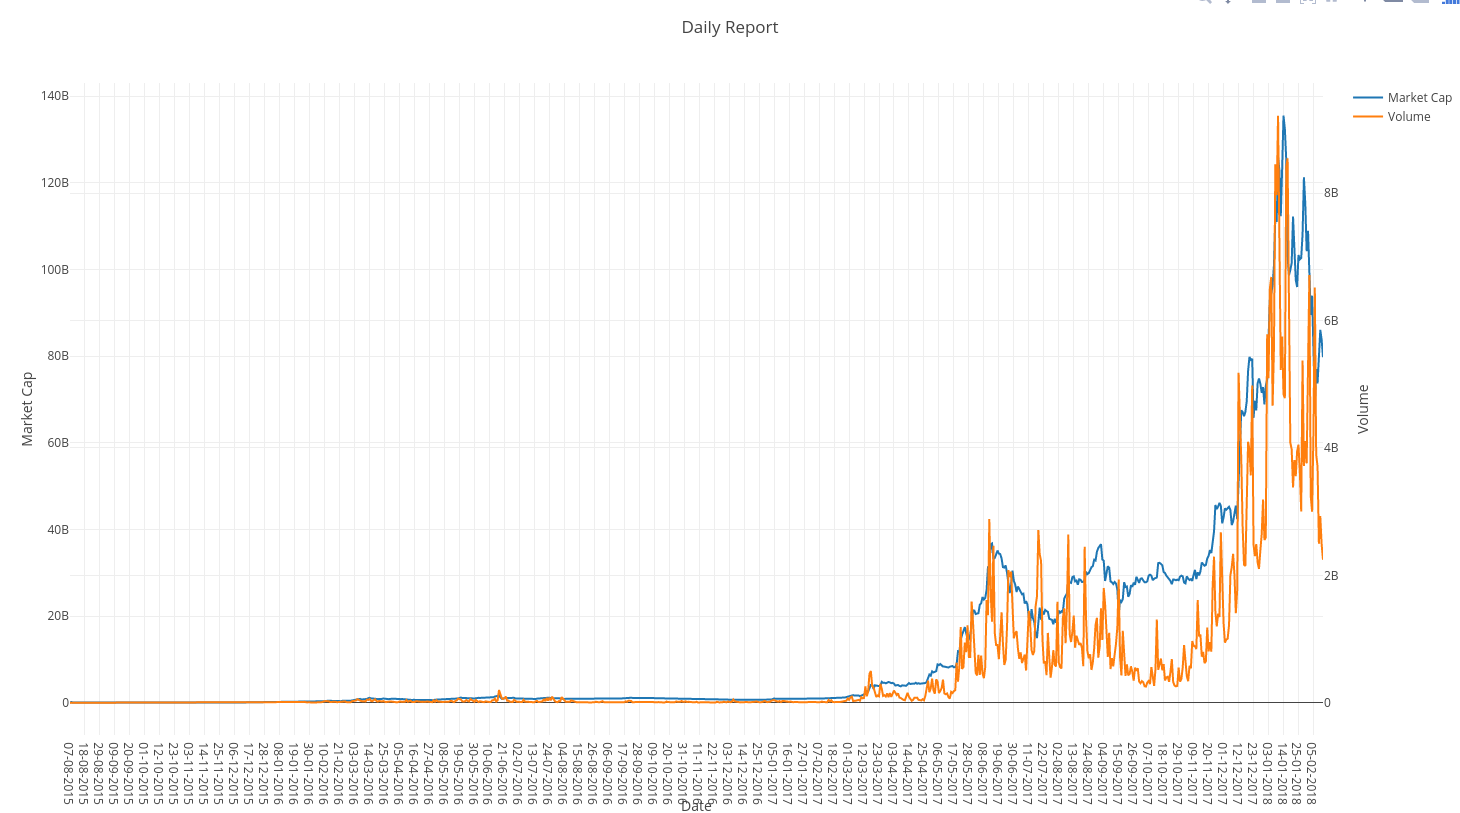
\includegraphics[trim=0 0 0 0.5cm, clip, scale=0.2]{price_daily.png}
    \]
\end{center}
If we set the query in order to retrieve the weekly and monthly mean of this information, we have the following graphics:
\begin{center}
    \[
        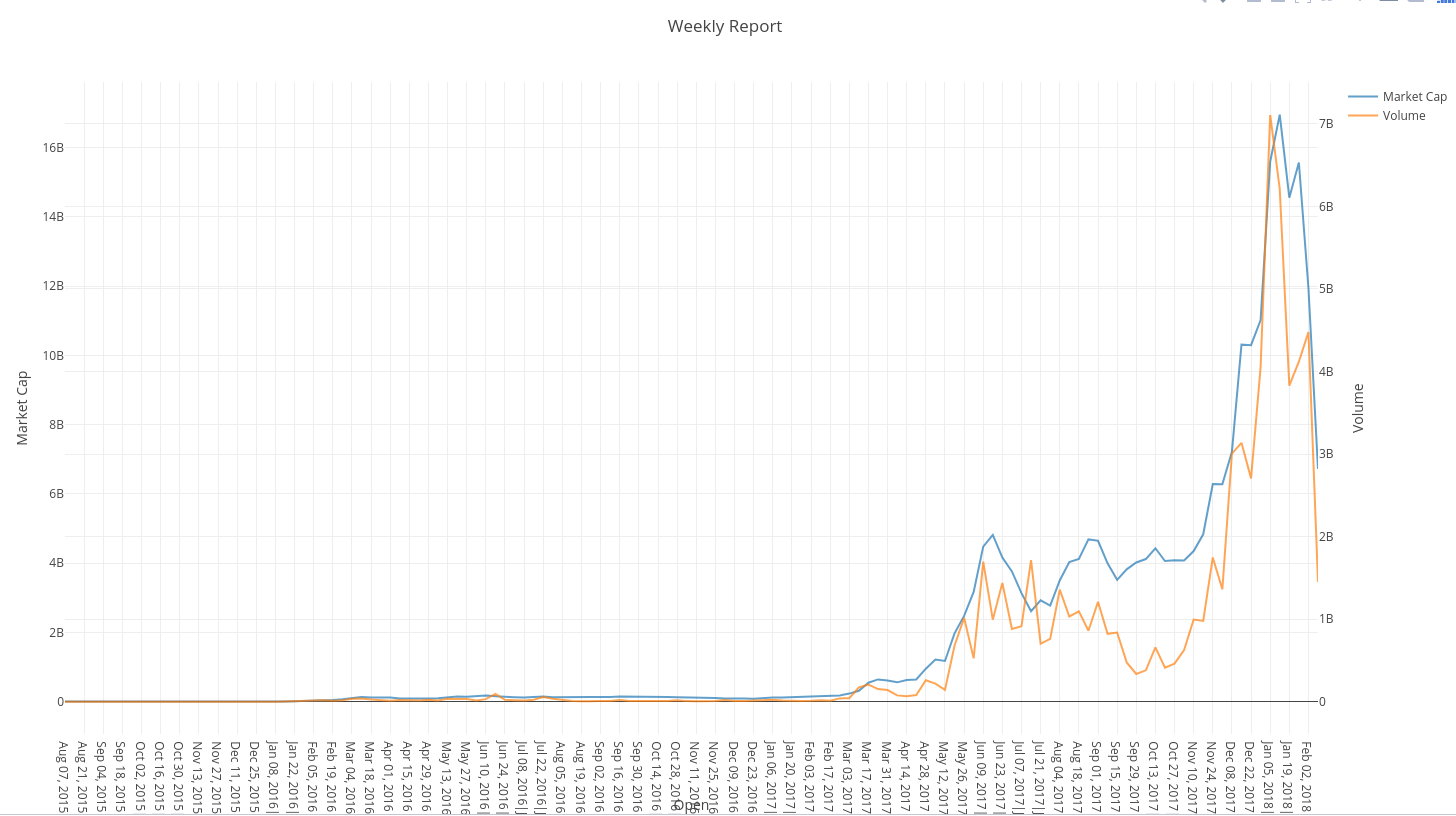
\includegraphics[trim=0 0 0 0.5cm, clip, width=0.5\columnwidth]{price_weekly.png}
        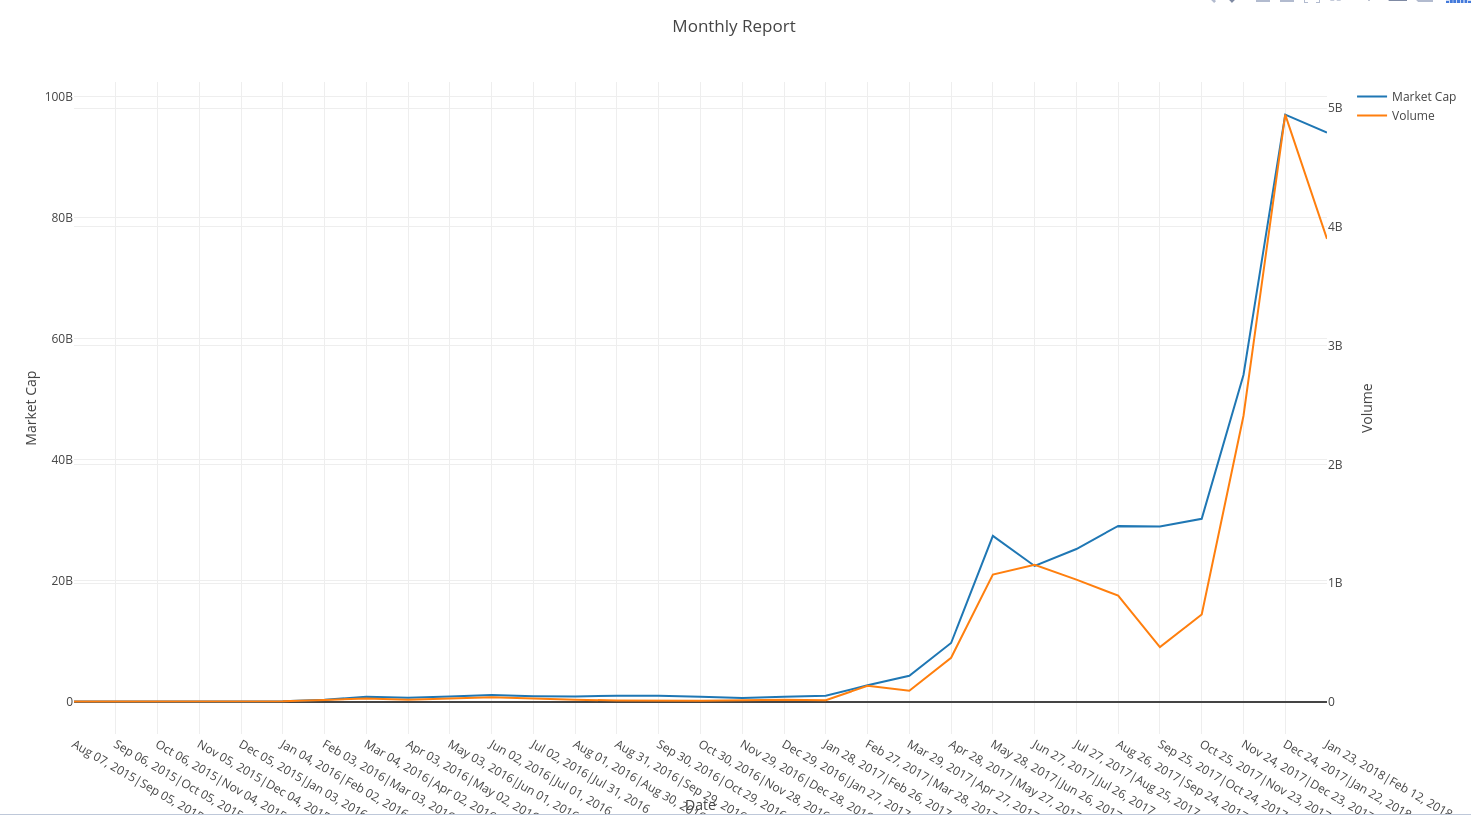
\includegraphics[trim=0 0 0 0.5cm, clip, width=0.5\columnwidth]{price_monthly.png}
    \]
\end{center}
\section{Case study: Levenshtein Distance between contract}
In information theory, Linguistics and computer science, the Levenshtein distance is a string metric for measuring the difference between two sequences.
In order to calculate Levenshtein distance between contracs EVM, first of all we create a view in MongoDB or SQL that contains only useful information retrieved from blockchain.
The useful fields are only two:
\begin{itemize}
    \item \textit{\textbf{contractAddress}}: The contract address inside blockchain (to uniquely identify a contract inside view);
    \item \textit{\textbf{contractCode}}: The contract EVM code
\end{itemize}
The distance calculation is done using this formula:
\begin{center}
$\operatorname{lev}_{a,b}(i,j) = 
\begin{cases}
  \max(i,j) & \text{ if} \min(i,j)=0, \\
  \min \begin{cases}
      \operatorname{lev}_{a,b}(i-1,j) + 1 \\
      \operatorname{lev}_{a,b}(i,j-1) + 1 \\
      \operatorname{lev}_{a,b}(i-1,j-1) + 1_{(a_i \neq b_j)}
   \end{cases} & \text{ otherwise.}
\end{cases}
$
\end{center}

\section{Case Study: Collection of ICOs data}
In order to store blockchain data combined with the external data retrieved using functions described in section \ref{informationsources}, we chose to use SQL, for the sake of precision, we used PostgreSQL.
In the following section we will explain in details this view, and how we used it.
\subsection{ICO's View}
The view is composed of four SQL tables: 
\begin{outline}
    \1 \textit{Block}: contains all information about blocks retrieved directly from blockchain. In particularly, it contains the following columns:
        \2 \textit{Hash}: the block hash inside blockchain, which is an unambiguous 32-Byte value and is used as table primary key;
        \2 \textit{Number}: represents the block's order inside blockchain;
        \2 \textit{Parent Hash}: contains the hash of the previous block, considered as its father inside blockchain;
        \2 \textit{Timestamp}: the date and time when this block is mined;
        \2 \textit{Miner}: the account that has mined this block;
    \1 \textit{Transaction}: contains all information about transaction contained inside every block, retrieved directly from blockchain. In particularly, it contains the following columns:
        \2 \textit{Hash}: the transaction hash inside blockchain, which is unambiguous like block ones and is used as table primary key;
        \2 \textit{nonce}: the number of transactions made by the sender prior to this one;
        \2 \textit{transaction index}: the number of this transaction inside its block;
        \2 \textit{from}: the transaction sender's address;
        \2 \textit{to}: the transaction receiver's address;
        \2 \textit{value}: value transferred in this transaction, in Wei;
        \2 \textit{creates}: this field is filled i and only if this transaction creates a contract. It contains the address of the newly created contract;
        \2 \textit{gas}: gas provided by the sender;
        \2 \textit{gasprice}: gas price provided by the sender in Wei;
        \2 \textit{blockhash}: the hash of the block that contains this transaction, it is used as the foreign key for the \textit{Block} table.
    \1 \textit{Internal-Transaction}
        \2 \textit{Id}: this field is used as primary key in this table;
        \2 \textit{Parent Tx Hash}: the hash of the father transaction. that is the transaction that generates this internal transaction;
        \2 \textit{Transaction type}: the internal transaction type (a value between call, suicide, create);
        \2 \textit{From}: the internal transaction sender's address;
        \2 \textit{To}: the internal transaction receiver's address;
        \2 \textit{Value}: alue transferred in this transaction, in Wei;
    \1 \textit{ICO}
        \2 \textit{Id}: this field is used as primary key in this table;
        \2 \textit{Token Name}: The token name;
        \2 \textit{Token Symbol}: The token Symbol;
        \2 \textit{Contract Address}: the address of the ERC20-contract that has created this token;
        \2 \textit{Market Cap}: The token market capitalization;
        \2 \textit{Total Supply}: The token total supply;
        \2 \textit{Price USD}: The current token price (USD);
        \2 \textit{Price BTC}: The current token price (BTC);
        \2 \textit{Hype Score}: The token hype score, given by ICORating;
        \2 \textit{Risk Score}: The token risk score, given by ICORating;
        \2 \textit{Investment Rating}: The token investment rating, given by ICORating;
        \2 \textit{Tx Creator Hash}: The address of the transaction that has created the ERC20-contract, which address is in the \textit{Contract Address} field.
\end{outline}

\section{Examples of tool usage on ICOs}
In this view we stored all data contained beetween block 3000000 and block 4100000, these are the block mined in the first seven month of 2017.
We collect data about:
\begin{itemize}
    \item 1.100.000. Blocks;
    \item About 22.000.000 Transactions;
    \item 4.000.000 Internal transactions;
    \item 1.500 ICOs
\end{itemize}
In this section, we discuss some studies done with all this data, stored in a SQL database.
\subsection{MarketCap and Volume with Exchange Rates}
With all information retrieved on \textit{CoinMarketCap} and \textit{CryptoCompare}, we can extract the historical exchange rate of all tokens, and combine them with transaction data in order to retrieve Market Capitalization and Volume of each token.
\newline
In this example, we examinate the historical Volume and Historical Market Capitalization of one ICO: 0x (ZRX).
\newline
Insert here query to retrieve transaction data about 0x.

\section{Performance}

\section{Conclusions and future works}
We have presented a framework for developing general-purpose analytics on the Ethereum blockchain and his ICOs. Its main component is a Scala library which can be used to construct views of the blockchain, possibly integrating blockchain data with data retrieved from external sources. Blockchain views can be stored as SQL or NoSQL databases, and can be analysed by using their query languages. Our experiments confirmed the effectiveness and generality of our approach, which uniformly comprises in a single framework several use cases addressed by various ad-hoc approaches in literature. Indeed, the expressiveness of our framework overcomes that of the closer proposals in the built-in support for external data, and the support of different kinds of databases and blockchains.
Importantly, coming in the form of an open source library for a mainstream language, our framework is amenable of being validated and extended by a community effort, following reuse best practices.

On the comparison of SQL vs NoSQL, our experiments did not highlight significant differences in the complexity of writing and executing queries in the two languages. Instead, we observed that the schema-less nature of NoSQL databases simplifies the Scala scripts.

A more accurate analysis, carried over a larger benchmark, is scope for future work. Anyway, it is worth recalling that the goal of our proposal is provide to the final user the flexibility to choose the preferred database, rather than ascertain an idea of best-fit-for-all in the choice.